%=====================================================
%====== If you are new to LaTeX, this website ========
%======     will be your new best friend:     ========
%======   http://en.wikibooks.org/wiki/LaTeX  ========
%======   Template created by Jonathan Blair  ========
%=====================================================



%=====================================================
%============ Controls ===============================
%=====================================================

%\documentclass[12pt,letterpaper,onecolumn]{article}
\documentclass[11pt,letterpaper,onecolumn]{article}
%\documentclass[10pt,letterpaper,onecolumn]{article}  % not recommended
%\documentclass[12pt,letterpaper,twocolumn]{article}
%\documentclass[11pt,letterpaper,twocolumn]{article}
%\documentclass[10pt,letterpaper,twocolumn]{article}


\usepackage{amsmath}
\usepackage{graphicx}
\usepackage{url}
\usepackage{textgreek}
\usepackage{float}
\usepackage{booktabs}
%\graphicspath{{path-to-folder-containing-necessary-graphics}{other folder as necessary}}


%=====================================================
%============ \begin{document} =======================
%=====================================================

\begin{document}

%=====================================================
%============ Title ==================================
%=====================================================

\title{\bf Observation of the Behavior of an Operational Amplifier}
%\title{\Large\bf Larger, Bolded Title}

%=====================================================
%============ Author =================================
%=====================================================
\author{
 Jairo Portillo \\*
  \\*
 PHY 338K Electronic Techniques \\*
 Department of Physics \\*
 The University of Texas at Austin \\*
 Austin, TX 78712, USA
}
\date{March 30, 2016}

%\address{The University of Texas, Austin, Texas, 78712}

\maketitle

%=====================================================
%============ Abstract ===============================
%=====================================================

\begin{abstract}

In this lab, we will explore the behavior of a Operational Amplifier as an inverting amplifier. We will measure the frequency response of the output and how the amplifier influences differentiation and integration of the input. We also observed the behavior of a summing amplifier with two function generators.

\end{abstract}

%=====================================================
%============ Body of the article ==========================
%=====================================================

%=====================================================
%============ Section ==================================
%=====================================================

\section{Preperation}

We know that an op-amp has two inputs an inverting and non-inverting. These inputs influence how our input signal will be given as an output. The amp also has power supply connections which are not usually visible on op-amp schematics. Op-amps typically always use feedback loops since they have a large voltage gain.   
For an inverting amplifier we know that the input impedance is 
$$Z_{in}=R_1}$$ 
and the gain 
$$G_V=-\frac{R_2}{R_1}$$
If we use a non-inverting the gain would have been
$$G_V = 1+\frac{R_2}{R_1}$$
which would put the signal well beyond the scope of the oscilloscope.  



\section{Lab work}

\subsection{Apparatus}

\begin{figure}[H]
    \centering
    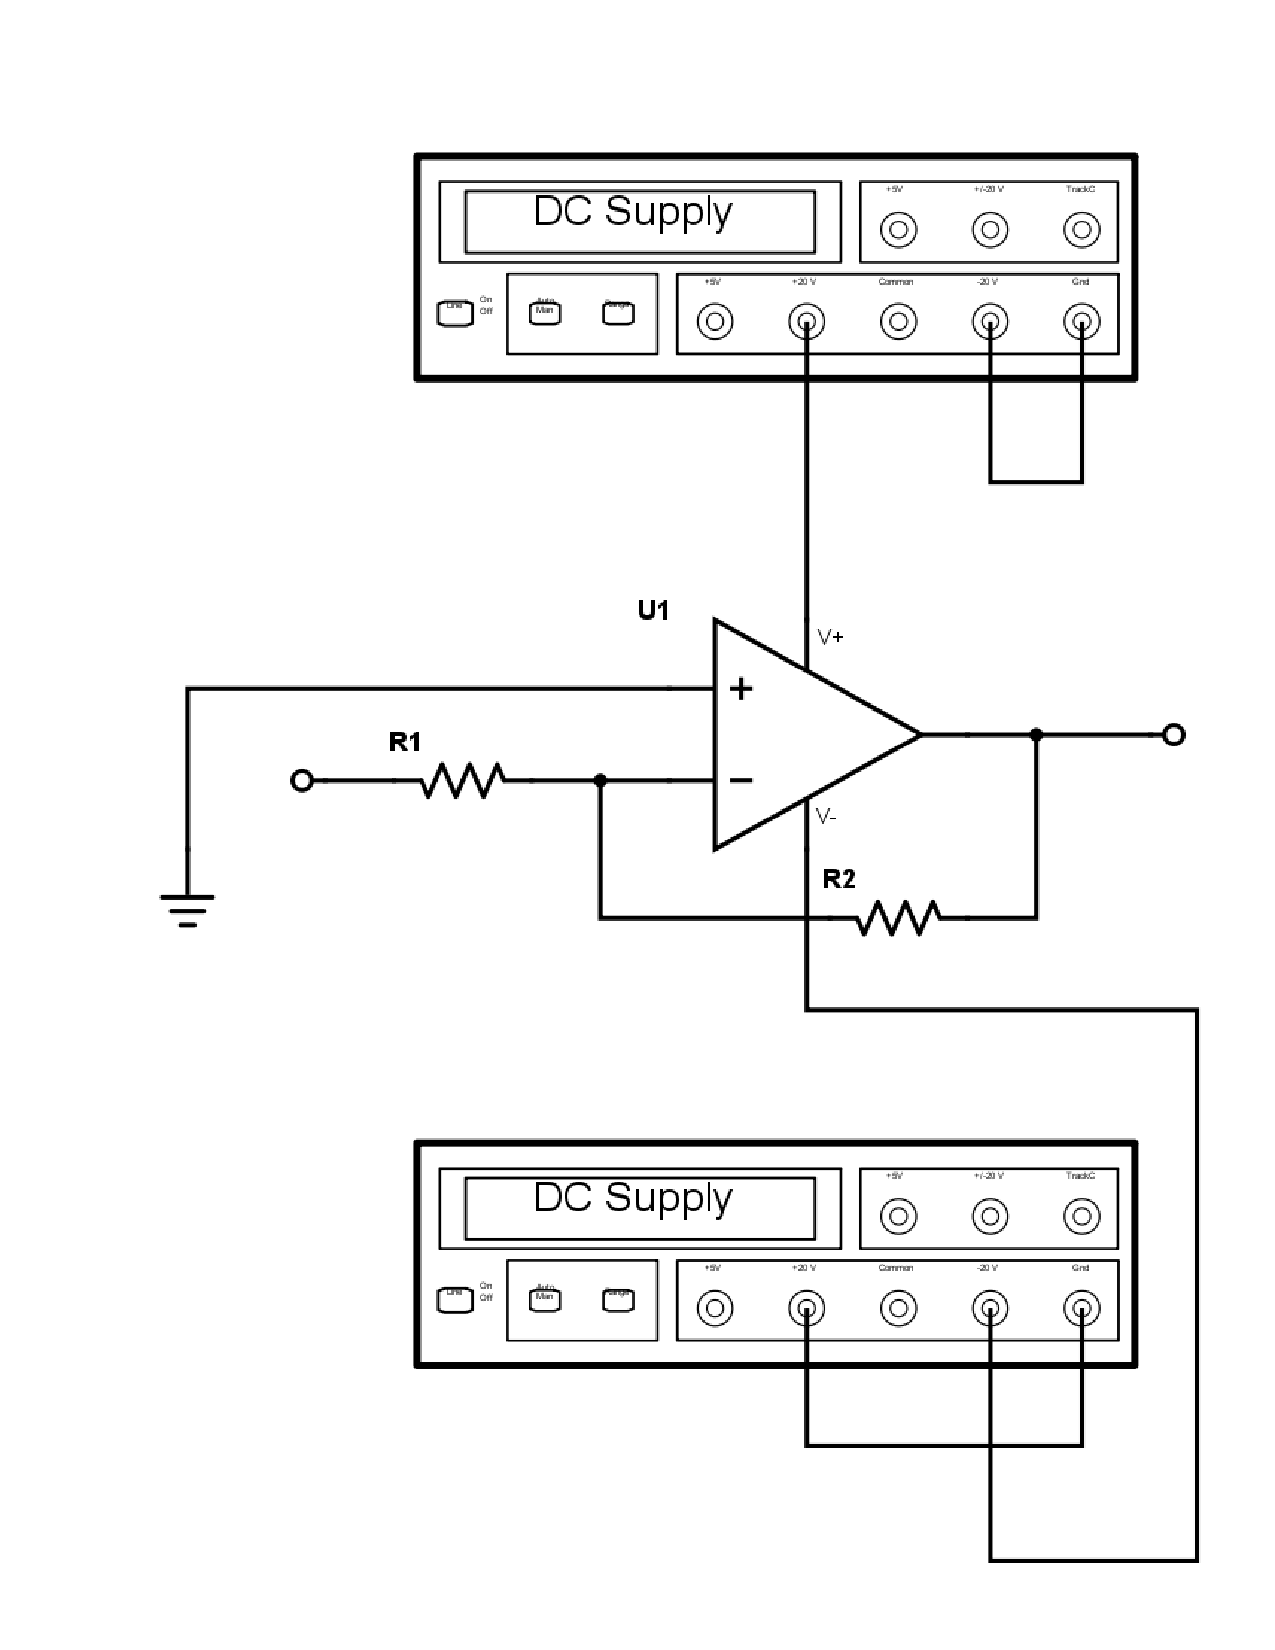
\includegraphics[scale = .5]{circuit.pdf}
    \caption{Our Op-amp amplifing circuit. $R_2$ will vary between 102.7 k$\Omega$ or 529 k$\Omega$ resistors.}
    \label{fig:cir}
\end{figure} 

This lab will use a signal generator, an oscilloscope, two DC voltage source, an op-amp, a 10 k$\Omega$, 102.7 k$\Omega$, and 529 k$\Omega$.A Tee connector will connect the input AC signal with channel 1 on the oscilloscope. The non-inverting input will be grounded. The AC signal generator will be in series with the 10 k$\Omega$ resistor and inverting input of the amp. It will also form a feedback loop with the output using the 102.7 k$\Omega$ or 529 k$\Omega$ resistors. The two DC supplies will each be given a specific voltage. One with give +15 V with the negative lead grounded and the other -15 V with the positive lead grounded. The to grounded leads will be connected and behave as our ground. A representation of our circuit can be seen in Figure 1.  



\subsection{Data Collection}

\begin{figure}[H]
    \centering
    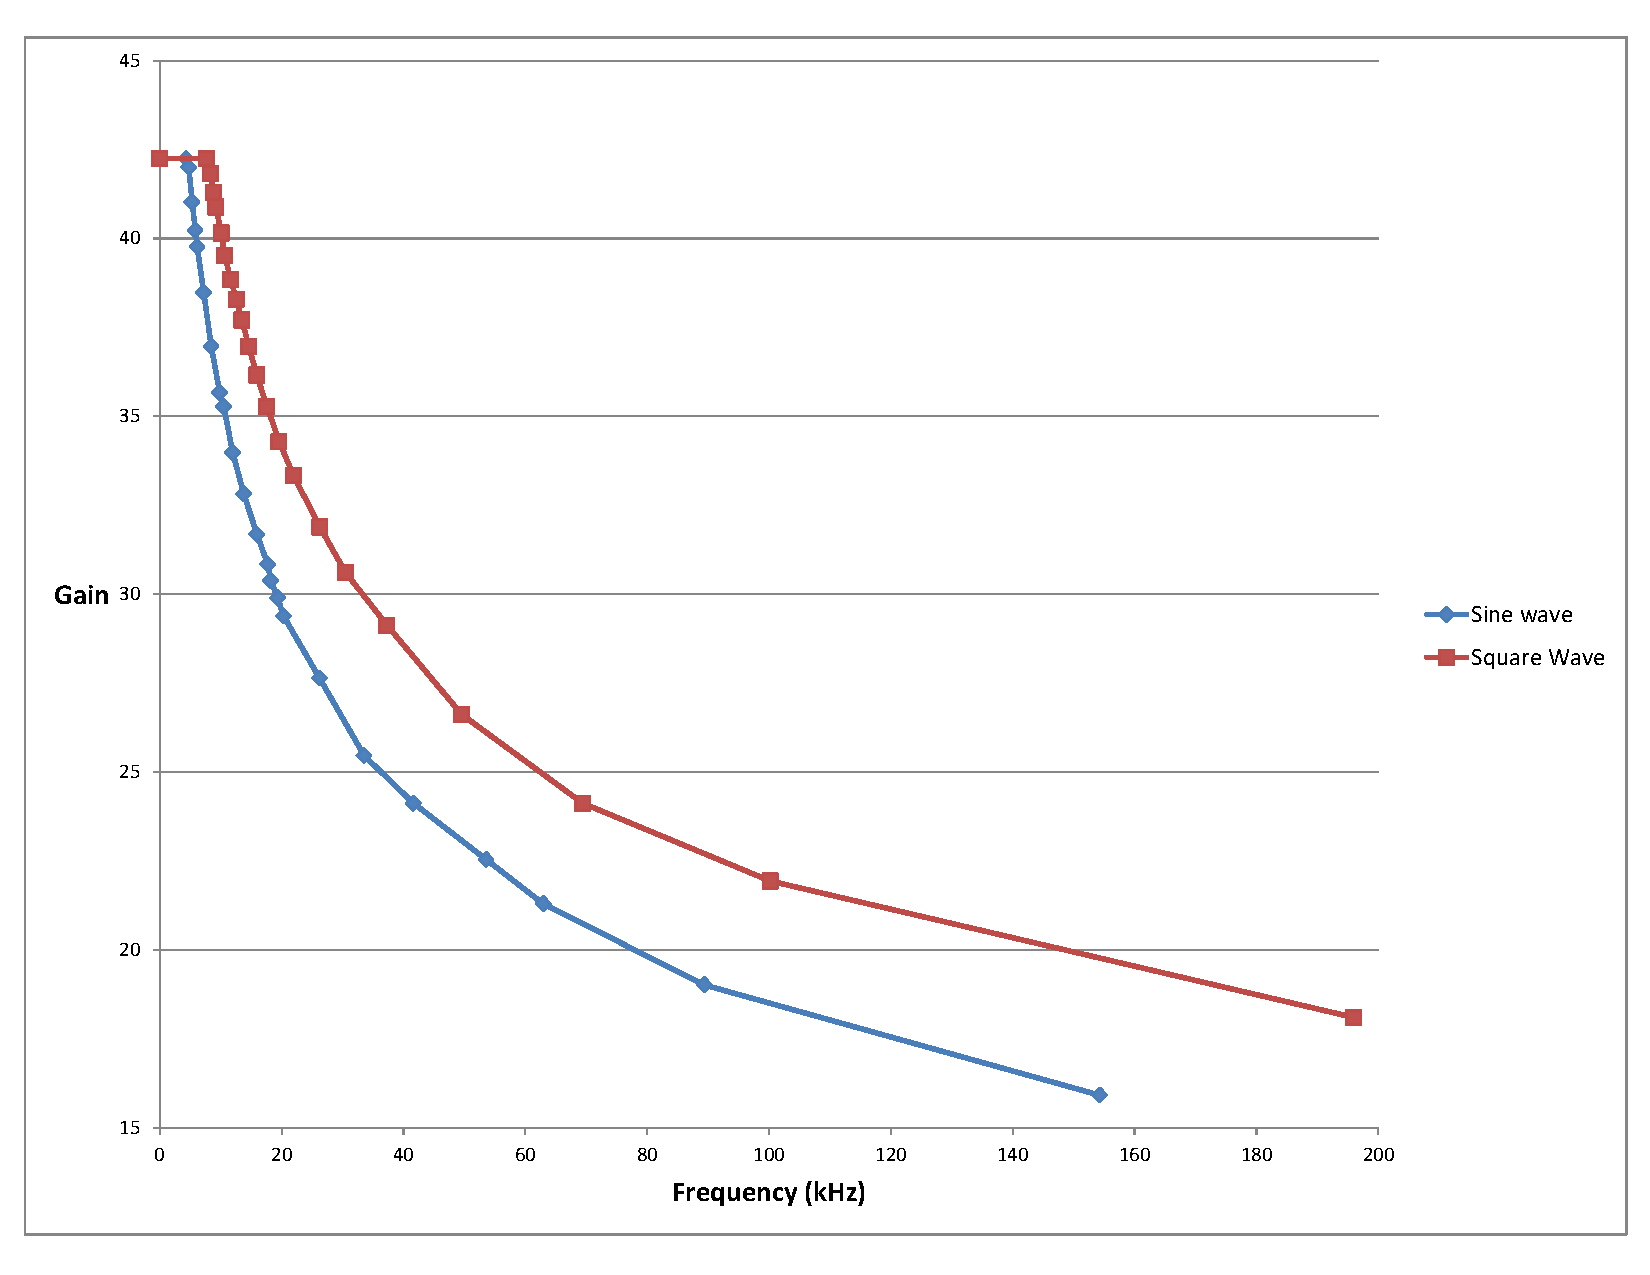
\includegraphics[scale = .5]{Graph1.pdf}
    \caption{The Gain vs Frequency for a square and sine wave.}
    \label{fig:grph1}
\end{figure}

For an inverting amplifier as we can see from Figure 2, that from 0 to 4kHz the sine input has a flat gain and until 5 kHz the gain begins to decrease as frequency increases. For the square wave the gain is stable from 0 to 8 kHz where it then begins to fall off. The input that was used was 224 mV since an input any higher would yield and output that would exceed the limits of the oscilloscope. 

\begin{figure}[H]
    \centering
    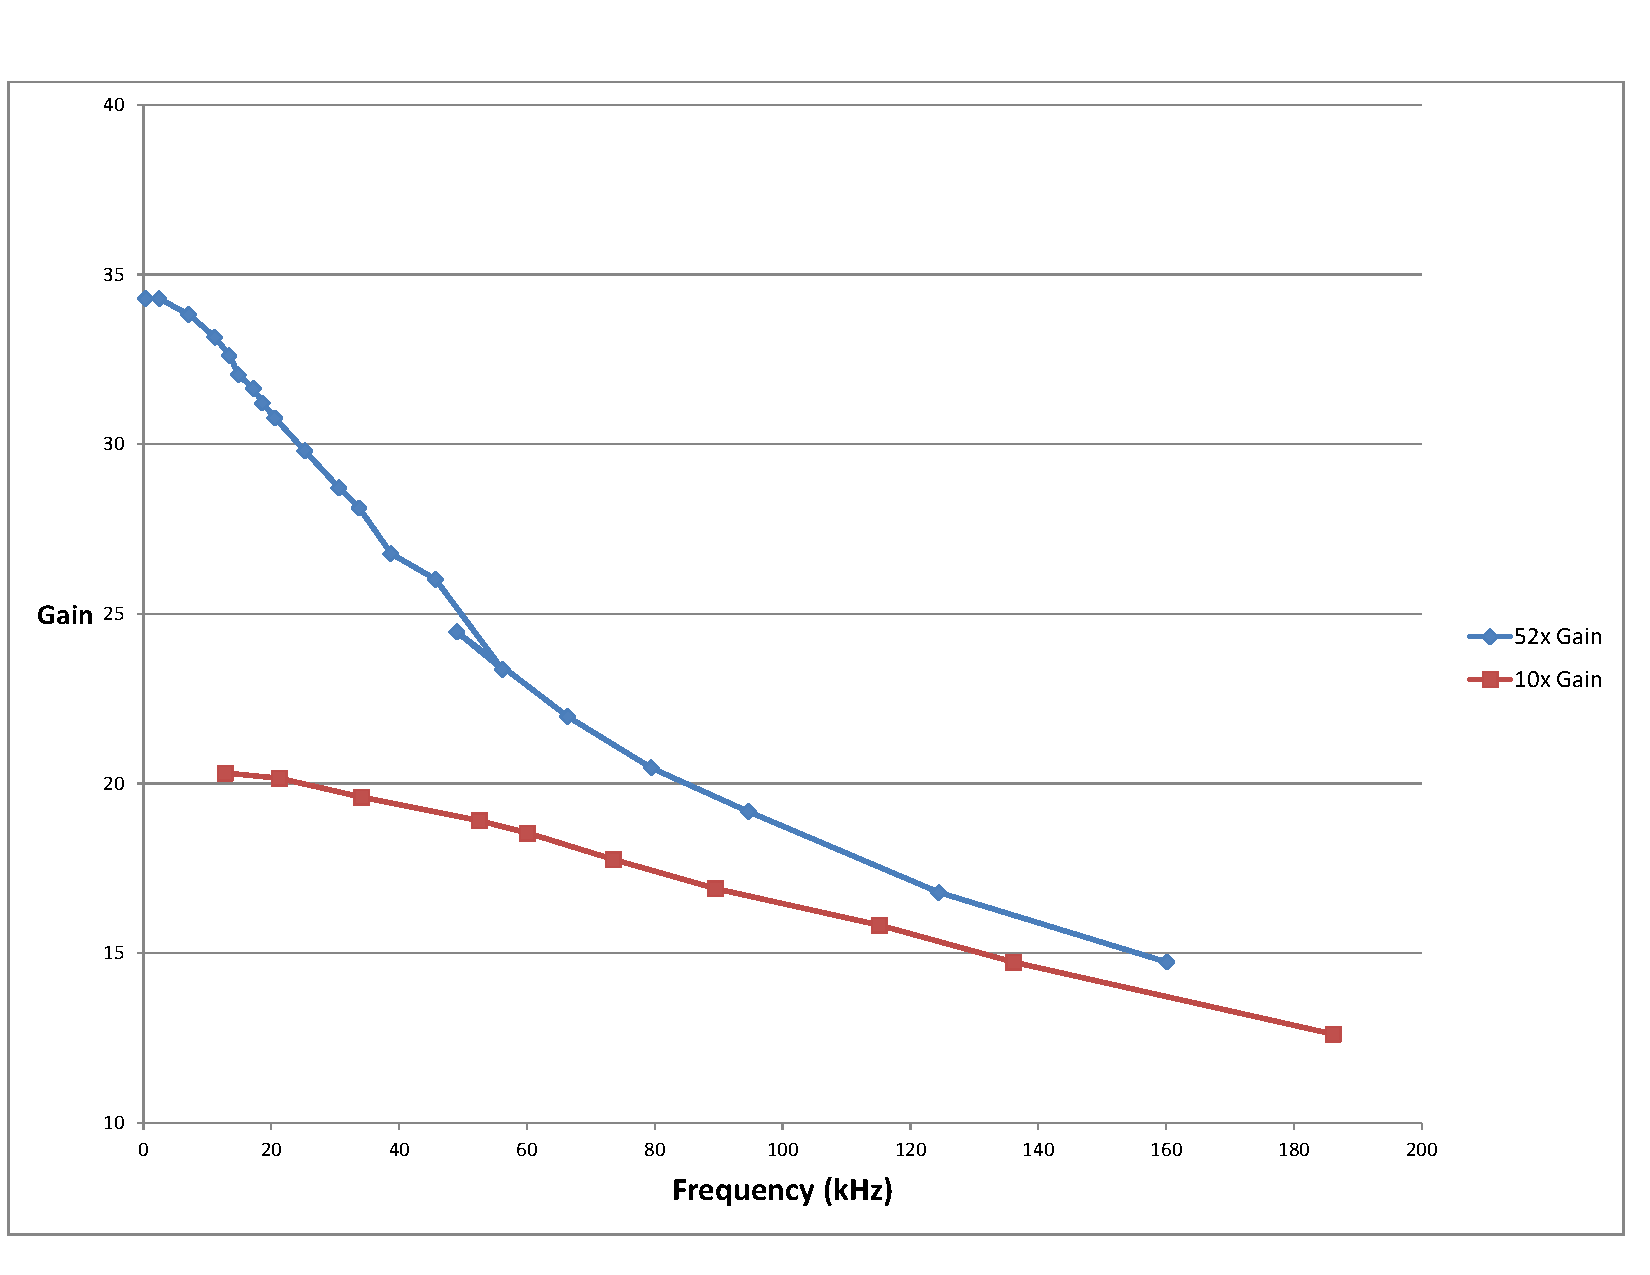
\includegraphics[scale = .5]{Graph2.pdf}
    \caption{The Gain vs Frequency for a gain of 52 and a gain of 10}
    \label{fig:grph2}
\end{figure}

From Figure 3 we can see that the higher the gain the faster the gain decreases as the frequency increases. The circuit used to find this plot is seen in Fig 1. The blue line in Fig 3 uses an $R_2$ of 529 k$\Omega$ while the red line uses the 102.7 k$\Omega$ resistor. Both use an $R_1$ of 10 k$\Omega$. 

\begin{figure}[H]
    \centering
    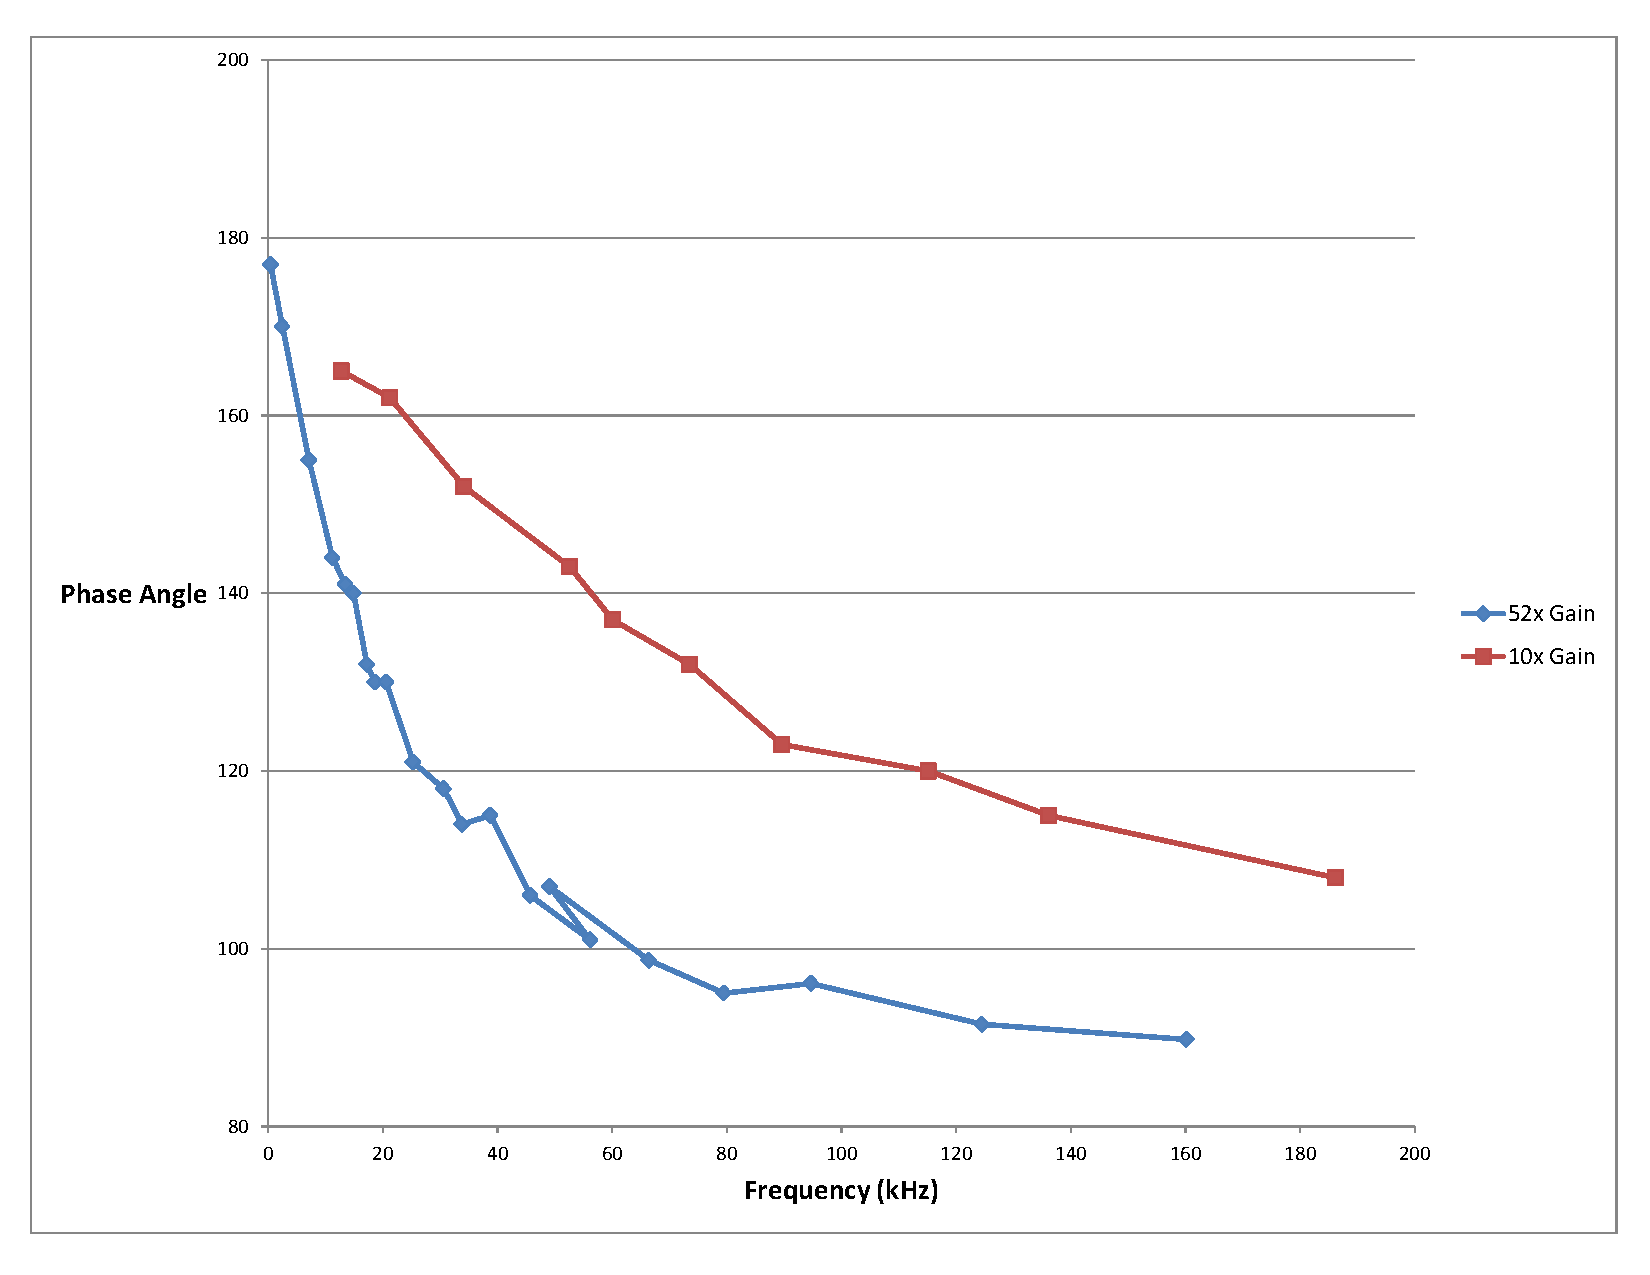
\includegraphics[scale = .5]{Graph3.pdf}
    \caption{The Phase difference vs Frequency for a gain of 52 and a gain of 10}
    \label{fig:grph3}
\end{figure}

The phase difference followed a similar patter as the gain behavior for both gains. At a higher maximum gain the the rate at which the gain and phase fall increases as frequency increases. This effect is seen but not as drastically in the 10x gain compared to the 52x gain. 

\section{Summary and conclusions}

In this lab, we have seen how an operational amplifier can amplify signal and how the amplification varies with frequency. From Fig 3, we can see how gain increases as frequency decreases and from Fig 4 the same relationship can be seen with the phase. Both graphs also demonstrated that at a higher maximum gain the rate of decreasing increases relative to frequency. 



%=====================================================
%============ Bibliography  ==============================
%=====================================================



%=====================================================
%============ End ====================================
%=====================================================

\end{document}

%=====================================================
%============ End ====================================
%=====================================================